\newpage
\section{Ganze Zahlen $\mathbb{Z}$}

Die natürlichen Zahlen sind unter Addition und Multiplikation abgeschlossen: Addieren und multiplizieren wir natürliche Zahlen, so ist das Ergebnis wieder eine natürliche Zahl. Für die Subtraktion funktioniert das leider nicht. Rechnen wir
\[
  5-7 = \square
\]
so können wir mit den natürlichen Zahlen kein Ergebnis finden.

Denken wir an die Äpfel zurück: wir können von fünf Äpfeln nicht sieben wegnehmen, da wir nicht weniger als null Äpfel haben können.

In der Tat haben sich auch berühmte Mathematiker lange gegen negative Zahlen gesträubt. Sie bekamen dann aber zum Rechnen mit Schulden einen praktischen Nutzen.

Wenn man von fünf Äpfeln sieben Äpfel abziehen möchte, ist die Frage: «Wie viele Äpfel bräuchte es noch, damit am Ende alle Äpfel weg sind?». Die Antwort ist Zwei! Rechnen wir $5-7$ so erhalten wir das Gegenteil von Zwei (bzgl. der Addition), also Minus Zwei!
\[
  5-7 = -2
\]

% ----------------------------------------------------------------------------
\subsection{Definition: Gegenzahl}

Welche Zahl muss zu Fünf addiert werden, um Null zu erhalten?
\[
  5 + \square = 0
\]
Wenn nur die natürlichen Zahlen betrachtet werden, gibt es keine Antwort auf diese Frage. Wenn in der Mathematik eine Lücke entdeckt wird, dann wird oft etwas neues definiert, das heisst «erfunden», um diese Lücke zu füllen.

In diesem Fall werden neue Zahlen definiert, welche diese Gleichung erfüllen.

\textbf{Definition:} Eine Zahl, welche Null ergibt, wenn sie zu einer gegebenen Zahl $a$ addiert wird, wird \textbf{Gegenzahl} von $a$ genannt und mit $-a$ bezeichnet:
\[
  a + (-a) = 0
\]
Die Gegenzahl von $5$ ist also $-5$ und $5 + (-5) = 0$. Wird die Menge der natürlichen Zahlen um ihre Gegenzahlen erweitert, so ergibt sich die Menge der \textbf{ganzen Zahlen}.

\textbf{Definition:} Die Menge der ganzen Zahlen $\mathbb{Z}$ enthält sämtliche natürliche Zahlen sowie ihre Gegenzahlen.
\[
  \mathbb{Z} = \{\ldots -4, -3, -2, -1, 0, 1, 2, 3, 4, \ldots\}
\]
\textbf{Anmerkung:} Die Gegenzahl von $0$ ist wieder $0$, da $0+0 = 0$ gilt. Deshalb ist $-0 = 0$.

% ----------------------------------------------------------------------------
\subsection{Zahlengerade und Betrag}

Auch die ganzen Zahlen können auf der Zahlengeraden dargestellt werden. Dabei wird die Gegenzahl jeder Zahl gegenüberliegend der Null dargestellt. So wird die Zahl $-4$ auf der anderen Seite von Null mit gleichem Abstand zur Null wie die Zahl $4$ dargestellt.
\begin{center}
  \begin{tikzpicture}
    \tkzInit[xmin=-5.5,xmax=5.5]
    \tkzDrawX[label={}]
    \tkzLabelX
    \tkzDefPoint(0,0){O}
    \tkzDefPoint(-4,0){A}
    \tkzDefPoint(4,0){B}
    \tkzDrawSegment[dim={$4$,10pt,}](A,O)
    \tkzDrawSegment[dim={$4$,10pt,}](O,B)
  \end{tikzpicture}
\end{center}

Der Abstand einer Zahl $a$ zur Null auf der Zahlengerade wird als ihr Betrag $|a|$ bezeichnet.

\textbf{Definition:} Der \textbf{Betrag} $|a|$ einer negativen Zahl $a$ ist ist die Gegenzahl von $a$. Der Betrag $|a|$ einer nicht-negativen Zahl $a$ ist gleich $a$.
\[
  |a| := \begin{cases}
    a &\quad a \geq 0 \\
    -a &\quad a < 0
  \end{cases}
\]
\begin{example}
  \textbf{Beispiele:} $|-3| = 3 \qquad |4| = 4 \qquad |-4| = 4$
\end{example}

% ----------------------------------------------------------------------------
\subsection{Abgeschlossenheit}

Die ganzen Zahlen sind bezüglich der Addition, der Subtraktion und der Multiplikation abgeschlossen. Das bedeutet, dass die Summe, die Differenz und das Produkt zweier ganzen Zahlen immer eine ganze Zahl ist.

% ----------------------------------------------------------------------------
\subsection{Teilmengen}
Oft wird über bestimmte Teilmengen der ganzen Zahlen gesprochen. Dabei werden die folgenden Begriffe und Symbole verwendet:
\begin{center}
  \renewcommand{\arraystretch}{1.3}
  \begin{tabularx}{0.8\textwidth}{Xcl}
      \textbf{Begriff}           & \textbf{Symbol}  & \textbf{Menge} \\
    \toprule
      positive ganze Zahlen      & $\mathbb{Z}^{+}$   & $\{1, 2, 3, 4, \ldots\}$ \\
    \midrule
      nichtnegative ganze Zahlen & $\mathbb{Z}_{0}^{+}$ & $\{0, 1, 2, 3, 4, \ldots\} = \mathbb{N}$ \\
    \midrule
      negative ganze Zahlen      & $\mathbb{Z}^{-}$   & $\{\ldots, -4, -3, -2, -1 \}$ \\
    \midrule
      nichtpositive ganze Zahlen & $\mathbb{Z}_{0}^{-}$ & $\{\ldots, -4, -3, -2, -1, 0 \}$ \\
    \bottomrule
  \end{tabularx}
\end{center}

% ----------------------------------------------------------------------------
\subsection{Negative Zahlen und Gegenzahlen}

Es ist nicht so, dass Gegenzahlen immer negativ sind. Jede beliebige Zahl $a$ hat eine Gegenzahl, egal ob $a$ selbst positiv ist, oder nicht. Die Gegenzahl von $a = -5$ ist beispielsweise $-a = -(-5) = 5$.

Wenn eine Variable $a$ verwendet wird, um über eine beliebige Zahl zu sprechen, kann es also auch sein, dass die Gegenzahl $-a$ eine positive Zahl ist und zwar genau dann, wenn $a$ eine negative Zahl ist.

% ----------------------------------------------------------------------------
\subsection{Rechenregeln}

Für das Rechnen mit Gegenzahlen gelten die folgenden Rechenregeln:
\begin{theorem}
  \textbf{Gegen-Gegenzahl.} Die Gegenzahl der Gegenzahl einer Zahl ist die ursprüngliche Zahl:
  \[
    -(-a) = a
  \]
\end{theorem}
\begin{theorem}
  \textbf{Addition und Subtraktion.} Das Addieren der Gegenzahl ist das Gleiche wie das Subtrahieren der Zahl. Das Subtrahieren der Gegenzahl ist das gleiche wie das Addieren der Zahl.
  \[
    a+(-b) = a-b \qquad\qquad a-(-b) = a+b
  \]
\end{theorem}
\begin{theorem}
  \textbf{Subtraktion einer Summe.} Die Subtraktion einer Summe ist das Gleiche wie das Subtrahieren beider Summanden:
  \[
    a-(b+c) = a-b-c
  \]
\end{theorem}
\begin{theorem}
  \textbf{Subtraktion einer Differenz.} Die Subtraktion einer Differenz ist das Gleiche wie das Subtrahieren des Minuenden und das addieren des Subtrahenden.
  \[
    a-(b-c) = a-b+c
  \]
\end{theorem}
\begin{theorem}
  \textbf{Multiplikation von Gegenzahlen.} Für die Multiplikation von Gegenzahlen gelten folgende Regeln:
  \[
    (-a)\cdot b = a\cdot(-b) = -ab \qquad\qquad  (-a)\cdot(-b) = ab
  \]
\end{theorem}

\textbf{Anmerkung:} Wir haben gesehen, dass die Subtraktion nicht kommutativ ist, also $6-3\ne 3-6$. Mit Hilfe der Gegenzahlen können wir aber etwas tricksen, denn $6-3 = 6+(-3) = (-3)+6$.
